\chapter{IMU}

\section{Indroduction}

An Inertial Measurement Unit (IMU) is a device that consists of multiple sensors that measure linear acceleration, angular velocity, and magnetic field strength. These sensors are typically arranged in a specific pattern, such as a 3-axis accelerometer, 3-axis gyroscope, and 3-axis magnetometer. The IMU is used to measure the orientation, position, and movement of an object in 3D space.

IMUs are commonly used in a variety of applications, such as drones, robots, and virtual reality systems, where it is important to accurately measure the movement and orientation of the device. They are also used in smartphones and other portable devices to track the movement and orientation of the device for various applications, such as augmented reality, navigation, and gaming.
In general, they are used for: 

Orientation tracking:  to track the orientation of an object in space by using a combination of acceleration and angular velocity sensors. The data from these sensors can be used to calculate the orientation of the object using techniques like complementary filters or Kalman filters.

Motion sensing:  to detect motion and changes in acceleration. For example, an IMU in a smartphone can be used to detect when the phone is being shaken or moved.

Navigation: to navigate by combining data from the acceleration and angular velocity sensors with information from other sensors, such as GPS. 

IMU to a microcontroller or computer and write software to read the data from the sensors and perform the necessary calculations. There are also many libraries and software packages available that can simplify the process of working with IMUs.

IMUs can be classified into two main categories based on the type of sensors used: MEMS (microelectromechanical systems) IMUs and FOG (fiber optic gyro) IMUs. MEMS IMUs use small mechanical sensors that are etched onto a silicon chip, while FOG IMUs use optical fibers to measure angular velocity. MEMS IMUs are typically smaller and less expensive, but they are also less accurate and have a shorter lifespan compared to FOG IMUs.

\section{LSM9DS1 (Accelerometer, Gyroscope, and Magnetometre Sensor)}

The 9-axis inertial measurement unit (IMU) sensor present on the Arduino Nano 33 BLE sense has an accelerometre, gyroscope, and magnetic sensor. It measures , 3D linear acceleration, 3D angular Velocity and 3D magnetic field aroud the sensor. This 9-axis IMU sensor measures the Position, vibration, orientation and magnetic field around the sensor. To access the IMU data, you can use the built-in Arduino libraries, such as the "Arduino LSM9DS1" library for the LSM9DS1 IMU sensor on the Nano 33 BLE Sense. This library provides functions for reading the data from the accelerometer and gyroscope, as well as for converting the raw data into more meaningful values like pitch, roll, and yaw.    it is found under File > Examples > LSM9DS1 as shown in \ref{fig:Testware}.

\begin{figure}[htbp]
	\centering
	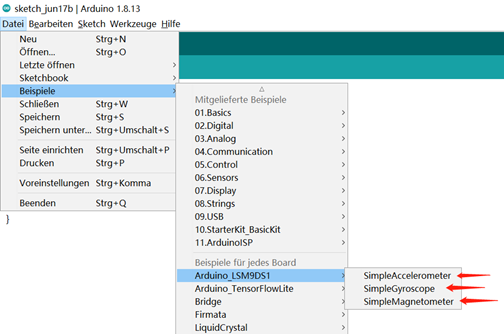
\includegraphics[width=7.5cm]{Images/Arduino/Testware3Sensoren}
	\caption{9-Axis IMU Sensor}
	\label{fig:Testware}
\end{figure}

After getting the results and output of the 9-axis IMU sensor, upload the available library program into the Arduino nano 33 BLE Sense.\\
To avoid any trouble during uploading the program, make sure to follow all the steps as we discussed in previous chapter e.g; (choose the board, select the port during upload and change the port when need to see output in serial monitor, reset arduino when needed).
Following uploading the program, results can be checked by opening the serial monitor as shown in figure.\ref{fig:IMU-Test} \\
Make sure to change the position and orientation of board and also place some Magnet aroud the borad, in order to see the changes on the outputed data.\\

\begin{figure}[htbp]
	\centering
	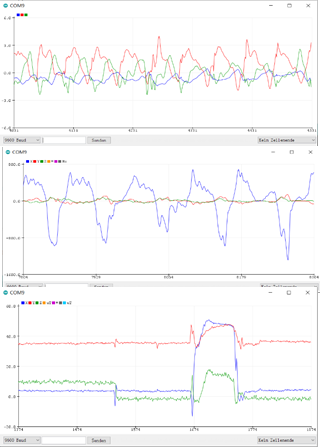
\includegraphics[width=7.5cm]{Images/Arduino/ErgebnisseIMUTests}
	\caption{Results of IMU-Tests}
	\label{fig:IMU-Test}
\end{figure}

The above 9-Axis IMU output \ref{fig:IMU-Test} , shows the 3-axis values for each accelerometer, gyroscope and magnetometer. These values changes as the sensor observes some changing in the sorroundings too, and it shows in the form of graph in the serial monitor. 

\section{Calibration}
%see https://www.youtube.com/watch?v=BLvYFXoP33o&ab_channel=FemmeVerbeek
It is important to calibrate an IMU since it ensures more accurate and precise measurements from the sensors. Without proper calibration, the measurements from the IMU may be affected by various sources of error, such as temperature, mechanical stress, or electromagnetic interference.\\
To calibrate the IMU, you can follow these steps:\\
1- Place the Nano 33 BLE Sense on a flat surface and make sure it is not moving.\\
2- Upload the following sketch to the Nano 33 BLE Sense:\\
\begin{verbatim}
#include <Arduino_LSM9DS1.h>

void setup() {
	Serial.begin(9600);
	while (!Serial);
	if (!IMU.begin()) {
		Serial.println("Failed to initialize IMU!");
		while (1);
	}
}

void loop() {
	IMU.readAcceleration(a[0], a[1], a[2]);
	IMU.readGyro(g[0], g[1], g[2]);
	IMU.readMag(m[0], m[1], m[2]);
	Serial.print("Acceleration: ");
	Serial.print(a[0]); Serial.print(" ");
	Serial.print(a[1]); Serial.print(" ");
	Serial.print(a[2]); Serial.print(" ");
	Serial.print("\tGyro: ");
	Serial.print(g[0]); Serial.print(" ");
	Serial.print(g[1]); Serial.print(" ");
	Serial.print(g[2]); Serial.print(" ");
	Serial.print("\tMag: ");
	Serial.print(m[0]); Serial.print(" ");
	Serial.print(m[1]); Serial.print(" ");
	Serial.println(m[2]);
	delay(100);
}

\end{verbatim}
3- Open the serial monitor in the Arduino IDE and set the baud rate to 9600.\\
4- Observe the raw accelerometer, gyroscope, and magnetometer readings for a few minutes.\\
5- Record the minimum and maximum values for each axis of the accelerometer and gyroscope.\\
6- Calculate the offsets for each axis by taking the average of the minimum and maximum values.\\
7- Subtract the offsets from the raw readings to obtain the calibrated readings.\\

For example, if the minimum and maximum values for the x-axis of the accelerometer are -100 and 100, respectively, the offset for the x-axis would be (100 + (-100)) / 2 = 0.\\

You can then use the calibrated readings in your code to obtain more accurate results.

Note: The magnetometer in our project will not be needed.
Even if it is a calibration isnt always required as the magnetometer is sensitive to the Earth's magnetic field, which is relatively stable. However, if you are using the magnetometer in a location with a strong local magnetic field, such as near a large metal object, you may need to calibrate it as well.




